%---------- Inleiding ---------------------------------------------------------

\section{Introductie} % The \section*{} command stops section numbering
\label{sec:introductie}

%Hier introduceer je werk. Je hoeft hier nog niet te technisch te gaan.
%
%Je beschrijft zeker:

%\begin{itemize}
%  \item de probleemstelling en context
%  \item de motivatie en relevantie voor het onderzoek
%  \item de doelstelling en onderzoeksvraag/-vragen
%\end{itemize}

Agile is een framework dat in het laatste decennium aan een grote opmars bezig is. Meer en meer bedrijven stappen af van een inflexibel watervalsysteem ten voordele van het flexibele en dynamische Agile framework. Momenteel behoort het tot de standaarden van de industrie. Binnen software development elimineert het enkele van de meest courante problemen die verantwoordelijk zijn voor het falen van veel software projecten.

Het valt te bemerken dat er een grote variatie bestaat in hoe de principes van Agile exact worden toegepast. Frameworks zoals Scrum en Kanban omvatten dezelfde principes met een andere uitwerking. In dit werk zal er geprobeerd worden te achterhalen wat de voor- en nadelen van 2 dergelijke workflows zijn en hoe deze gecombineerd kunnen worden teneinde een beter projectverloop. 

De vragen die in dit werk onderzocht zullen worden zijn:
\begin{itemize}
\item Welk effect heeft het werken in team aan een feature\footnote{Wanneer er naar 'werken in team' wordt verwezen zelfs al is de developer lid van een team, wordt hiermee altijd bedoeld dat er samen aan een feature of onderdeel wordt gewerkt, tenzij anders aangegeven.} op de vooruitgang van het project?
\item Welk effect heeft het werken in team op het welzijn van de developer (stress, etc.)?
\item Hoe kunnen beide workflows gecombineerd worden om het beste van beiden te bekomen en hoe vertaalt zich dat praktisch naar een framework?
\end{itemize}

%---------- Stand van zaken ---------------------------------------------------

\section{Stand van zaken}
\label{sec:state-of-the-art}

%Hier beschrijf je de \emph{state-of-the-art} rondom je gekozen onderzoeksdomein. Dit kan bijvoorbeeld een literatuurstudie zijn. Je mag de titel van deze sectie ook aanpassen (literatuurstudie, stand van zaken, enz.). Zijn er al gelijkaardige onderzoeken gevoerd? Wat concluderen ze? Wat is het verschil met jouw onderzoek? Wat is de relevantie met jouw onderzoek?
%
%Verwijs bij elke introductie van een term of bewering over het domein naar de vakliteratuur, bijvoorbeeld~\autocite{Doll1954}! Denk zeker goed na welke werken je refereert en waarom.
%
%% Voor literatuurverwijzingen zijn er twee belangrijke commando's:
%% \autocite{KEY} => (Auteur, jaartal) Gebruik dit als de naam van de auteur
%%   geen onderdeel is van de zin.
%% \textcite{KEY} => Auteur (jaartal)  Gebruik dit als de auteursnaam wel een
%%   functie heeft in de zin (bv. ``Uit onderzoek door Doll & Hill (1954) bleek
%%   ...'')
%
%Je mag gerust gebruik maken van subsecties in dit onderdeel.

\subsection{Principes}
De principes waar Agile op rust zijn relatief simpel. Deze werden in 2001 besproken en uitgeschreven door een groep van 17 developers \autocite{Beck2001}. De voor dit werk relevante principes zijn (geparafraseerd en vertaald):
\begin{itemize}
  \item Omarm veranderende requirements
  \item Lever regelmatig werkende software
  \item Een constant tempo moet voor onbepaalde tijd vol te houden zijn
  \item Werkende software is een maat voor voortgang
\end{itemize}

%''Welcome changing requirements, even late in development. Agile processes harness change for the customer's competitive advantage''.

''Verwelkom verandering in eisen, ook laat in de ontwikkeling. Agile-processen benutten verandering als een competitief voordeel voor de klant''

 \autocite{Beck2001}. De klant is in staat om de processen van projecten te beheersen  aan de hand van on-site interactie en requirements geven de huidige noden van de eindgebruikers waarheidsgetrouw weer \autocite{Kumar2012}. Dit wordt gezien als het grootste voordeel van Agile ten opzichte van een klassiek watervalsysteem. Frequente communicatie met de opdrachtgever ('De klant') leidt tot een constante instroom van feedback. In combinatie met een ander voordeel ('Lever regelmatig werkende software', zie verder) is de analist beter in staat de wensen van de klant (of herzieningen hiervan) en de interpretatie van het ontwikkelingsteam ('De developers') gelijk te stellen (of hier zo dicht mogelijk bij te komen). Een bijkomend voordeel is hier dat er een constante herziening van het product is, wat zorgt dat foutopsporing sneller en gemakkelijk gebeurt \autocite{Imreh2011}.

%''Deliver working software frequently, from a couple of weeks to a couple of months, with a preference to the shorter timescale''
''Lever regelmatig werkende software op. Liefst iedere paar weken, hooguit iedere paar maanden''

\autocite{Beck2001}. Eén van de essenties van Agile werken, is het iteratief en incrementeel werken. In de praktijk vertaalt dit zich naar het werken in sprints, waarbij er een vaste, korte periode een voorafgeplande hoeveelheid werk verricht wordt, waarna er bekeken wordt hoe dit verliep en wat er aangepast moet worden. In combinatie met het vorige punt ('Omarm veranderende requirements') kunnen veranderende requirements makkelijk geïntegreerd worden. Er gebeurt immers regelmatig een herziening van het product, want bij elke sprint is er een testfase.


%``Agile processes promote sustainable development. The sponsors, developers, and users should be able to maintain a constant pace indefinitely''
''Agile processen bevorderen duurzame ontwikkeling. De opdrachtgevers, ontwikkelaars en gebruikers moeten een constant tempo eeuwig kunnen volhouden''

\autocite{Beck2001}. Hoewel het mogelijks het simpelste principe is, is het tevens één van de belangrijkste. Een tempo dat comfortabel vol te houden is, leidt tot een betere werkomgeving en logischerwijs ook een beter product. Bij Agile zijn de teams waarin gewerkt wordt zelfsturend. De overhead is beperkt tot een stand-up waarbij eerder naar voortgang wordt gekeken. Organisatorische problemen worden tijdens een retrospective (aan het einde van de sprint) besproken en eventueel verbetert op een manier waar de developers zelf mee akkoord gaan, wat de developers gemotiveerd houdt.

%``Working software is the primary measure of progress''
''Werkende software is de belangrijkste maat voor voortgang''

\autocite{Beck2001}. Een goede maat hebben is een vereiste om voortgang te kunnen meten. Waar een watervalmethode dit moeilijk maakt, zal bij Agile het iteratief en incrementeel werken leiden tot meer werkende stukken software. Elke feature wordt apart behandeld en aan het einde van de sprint is het de bedoeling dat deze ook afgewerkt zijn. In een ideale situatie (wat echter zelden voorkomt) is er na elke sprint een werkend product waarbij de features minstens minimaal afgewerkt zijn en bij volgende sprints verder aan gewerkt zal worden.

\subsection{Toepassing}
Het is logisch dat de implementatie en toepassing van deze principes anders zullen zijn afhankelijk van de grootte van het bedrijf en het team zelf. Uit de principes valt op dat het gebruik van Agile te vergelijken valt met change management. Zelfs buiten software development is het een bruikbaar systeem om met verandering om te gaan. 
``The concept of agile working has been adopted by many organizations which have realized that their hierarchical structures and lengthy decision-making processes are no longer fit for purpose in a world of complex and continuous change'' \autocite{Franklin2014}. Hier valt uit af te leiden dat kleinere bedrijven sneller geneigd zullen zijn om Agile te gebruiken, daar deze een minder strikte hiërarchie hebben. Uit \textcite{Salo2008} valt op dat het gebruik van Agile toeneemt met een toenemende bedrijfsgrootte. Deze toont een verandering in gedachtengoed. Waar vroeger Agile vooral voor kleinere bedrijven en projecten was, is het inmiddels een gevestigde waarde geworden. Ook binnen de zogenaamde 'Fortune 500'-bedrijven, waaronder bv. Alphabet Inc., moederbedrijf van Google LLC, wordt hiervan gebruik gemaakt. 

\subsection{Implementaties}
Zoals onder 'Principes' te bemerken valt, Agile is geen uniform framework. De exacte toepassing van deze principes wordt vastgelegd in aparte frameworks. Hiervan zal er slechts 1 worden besproken, daar het doel van dit werk is om de principes zelf onder de loep te nemen ongeacht welk framework er gebruikt wordt, maar het wel nuttig kan zijn om een concrete implementatie van deze principes te bekijken.
Er werd hiervoor gekozen voor Scrum, daar dit het meest courant is \autocite{Sutherland2007}.
Scrum is een Agile framework met een relatief simpele structuur. Er zijn drie rollen vastgelegd: de Product Owner, het team en de Scrummaster. De Product Owner is de klant. Deze persoon is tevens beheerder van de lijst van taken ('De product backlog'), bepaalt wat in welke volgorde moet gebeuren. Het team is verantwoordelijk voor het afleveren van het product. Deze groep is multidisciplinair en verantwoordelijk voor alle stappen in het ontwikkelingsproces, gaande van analyse tot de testing. De Scrummaster leidt het team doorheen het Scrumproces. Deze persoon voorziet eventuele trainingen en organiseert de vergaderingen. Hij fungeert als contactpersoon tussen het team en externen, maar is geen project manager.
De rituelen die bij Scrum gebruikt worden, zijn o.a. de daily stand-up, sprint planning en retrospective. De daily stand-up is een dagelijkse, korte vergadering waar men al rechtstaand binnen 10 minuten de to-do, doing en done van elk lid overloopt en eventuele problemen uitlegt en om hulp vraagt waar nodig. Aan het begin van elke sprint gebeurt er een sprint planning, waar het verloop van de komende sprint wordt uitgepland en taken verdeeld. Aan het eind van de sprint gebeurt er een retrospective, waar wordt teruggeblikt op de afgelopen sprint, wat er al dan niet verkeerd is gelopen en hoe dit verbeterd kan worden.


Veel bedrijven gebruiken echter geen vast framework en hanteren een eigen implementatie van de Agile principes. Dit kan zijn omdat het type project het niet toelaat, het team niet de juiste grootte of vorm heeft of de requirements duidelijk en onveranderlijk zijn \autocite{Naekki2011}. Het is dus noodzakelijk dat een bedrijf alle parameters in gedachten houdt, zoals de bedrijfscultuur, het type product en hoe change management gebeurt. Projecten kunnen falen doordat het gekozen systeem niet geoptimaliseerd is voor de developers.


%---------- Methodologie ------------------------------------------------------
\section{Methodologie}
\label{sec:methodologie}

%Hier beschrijf je hoe je van plan bent het onderzoek te voeren. Welke onderzoekstechniek ga je toepassen om elk van je onderzoeksvragen te beantwoorden? Gebruik je hiervoor experimenten, vragenlijsten, simulaties? Je beschrijft ook al welke tools je denkt hiervoor te gebruiken of te ontwikkelen.

\subsection{Verzameling data}
De data zal verzameld worden door middel van regelmatige enquête. Door de verschillende aard van de twee te onderzoeken workflows en verschillen in project scope, is het noodzakelijk om een correcte schaal te kiezen. Om dit te bewerkstelligen, is het genoeg om naar de structuur van Agile projecten te kijken. Het is een zekerheid dat er bij alle projecten in sprints zal gewerkt worden. Er zal dus per sprint en per week een enquête afgenomen worden die pijlt naar de voortgang van het project en het welzijn van de developer. Er zullen verschillende aspecten bekeken worden als variabelen om af te kunnen leiden of deze al dan niet een effect hebben op beiden. Ten slotte zal er gekeken worden welke aspecten een positieve invloed hebben en welke combinaties er mogelijk zijn.
De enquête zal worden afgenomen via een Google Form waarbij er voor de voortgang en het welzijn een 5-punt Likertschaal zal gebruikt worden, waarbij een score van 3 neutraal is (voortgang is zoals verwacht, welzijn is normaal), 1 zeer slecht is (sterk achter op schema, zeer veel stress) en 5 zeer goed (sterk voor op schema, welzijn is zeer goed). Tevens zal er extra gegevens gevraagd worden, zoals natuurlijk het type workflow (individueel - teamgebonden), bedrijfscultuur en mogelijke externe factoren die een invloed kunnen hebben op beiden (teamlid die wegvalt, persoonlijke problemen, etc.). Het gebruik van een Likertschaal zorgt ervoor dat de subjectiviteit van 'welzijn' en 'voortgang' toch enigzins objectief wordt, doordat ze vergeleken worden met de baseline van de developer zelf. 


De enquête zal bij een groot aantal developers worden afgenomen, zodat er genoeg data aanwezig is om elke variabele te kunnen isoleren bij de verwerking. Er wordt gericht op 10 bedrijven met een gemiddelde teamgrootte\footnote{Grootte van het team waarin samen aan een feature gewerkt wordt} van 5 developers, waardoor de steekproefgrootte rond 50 respondenten ligt.

De te extra onderzoeken variabelen zijn\footnote{Naast de vergelijking tussen de individuele en teamsgebonden workflow. De lijst is niet limitatief, noch zullen ze noodzakelijk allemaal gebruikt worden.}:
\begin{itemize}
\item Grootte van het team waarin samengewerkt wordt
\item Sprintduur in weken
\item Veranderlijkheid van requirements
\end{itemize}

\subsection{Verwerking data}
Het verwerken van de data zal neerkomen op het berekenen van de correlatie tussen de variabelen. Uit de dataset zullen er verschillende clusters worden verdeeld, zodat er steeds slechts één onafhankelijke variabele zal zijn. 
De verwerking zal gebeuren in R of Python. Hieruit zal een correlatie-coëfficient uit worden berekend. De interpretatie zal simpel zijn. Een correlatie boven een bepaalde threshold ($\pm 0.7$) zal een sterke correlatie aantonen. Bij een coëfficient tussen $\pm 0.3$ en $\pm 0.7$ zal er sprake zijn van een matige correlatie. Hierbij kan gekeken worden of meerdere variabelen samen een sterke correlatie bekomen.

%---------- Verwachte resultaten ----------------------------------------------
\section{Verwachte resultaten}
\label{sec:verwachte_resultaten}

%Hier beschrijf je welke resultaten je verwacht. Als je metingen en simulaties uitvoert, kan je hier al mock-ups maken van de grafieken samen met de verwachte conclusies. Benoem zeker al je assen en de stukken van de grafiek die je gaat gebruiken. Dit zorgt ervoor dat je concreet weet hoe je je data gaat moeten structureren.

Er wordt verwacht dat een individuele workflow een betere voortgang betekent, maar een lagere score voor het welzijn van de developer zal hebben. De grootte van het team zal omgekeerd evenredig zijn met de voortgang en het welzijn, m.a.w. grotere teams developers zullen meer stress ervaren en minder voortgang maken op het project. Een kortere sprintduur zal meer stress veroorzaken maar tevens voor veel voortgang zorgen. De mate van veranderlijkheid van requirements zal omgekeerd evenredig zijn met zowel de voortgang als het welzijn. Een verwachte dataset werd geplot in figuren 1 en 2. Hierbij werd voor de eenvoud enkel de voortgang en het welzijn bekeken. Andere variabelen zullen meegerekend worden, maar werden niet visueel voorgesteld.

Volgende figuren zijn louter een visuele voorstelling van een mogelijke dataset. Het aantal punten die samenvallen worden niet speciaal weergegeven. De data van developers die individueel werken werd voorgesteld in figuur 1, voor zij die in team werken is dit in figuur 2. Hier werd de voortgang geplot in functie van het welzijn. De assen stellen de waarden voor, waar 3 een neutrale baseline is, 1 zeer slecht en 5 zeer goed is. Een kleurencode werd gebruikt om te punten visueel een score te geven, waarin rood een slechte situatie voorstelt, blauw een neutrale en groen een goede situatie.

\begin{figure}[!hb]
    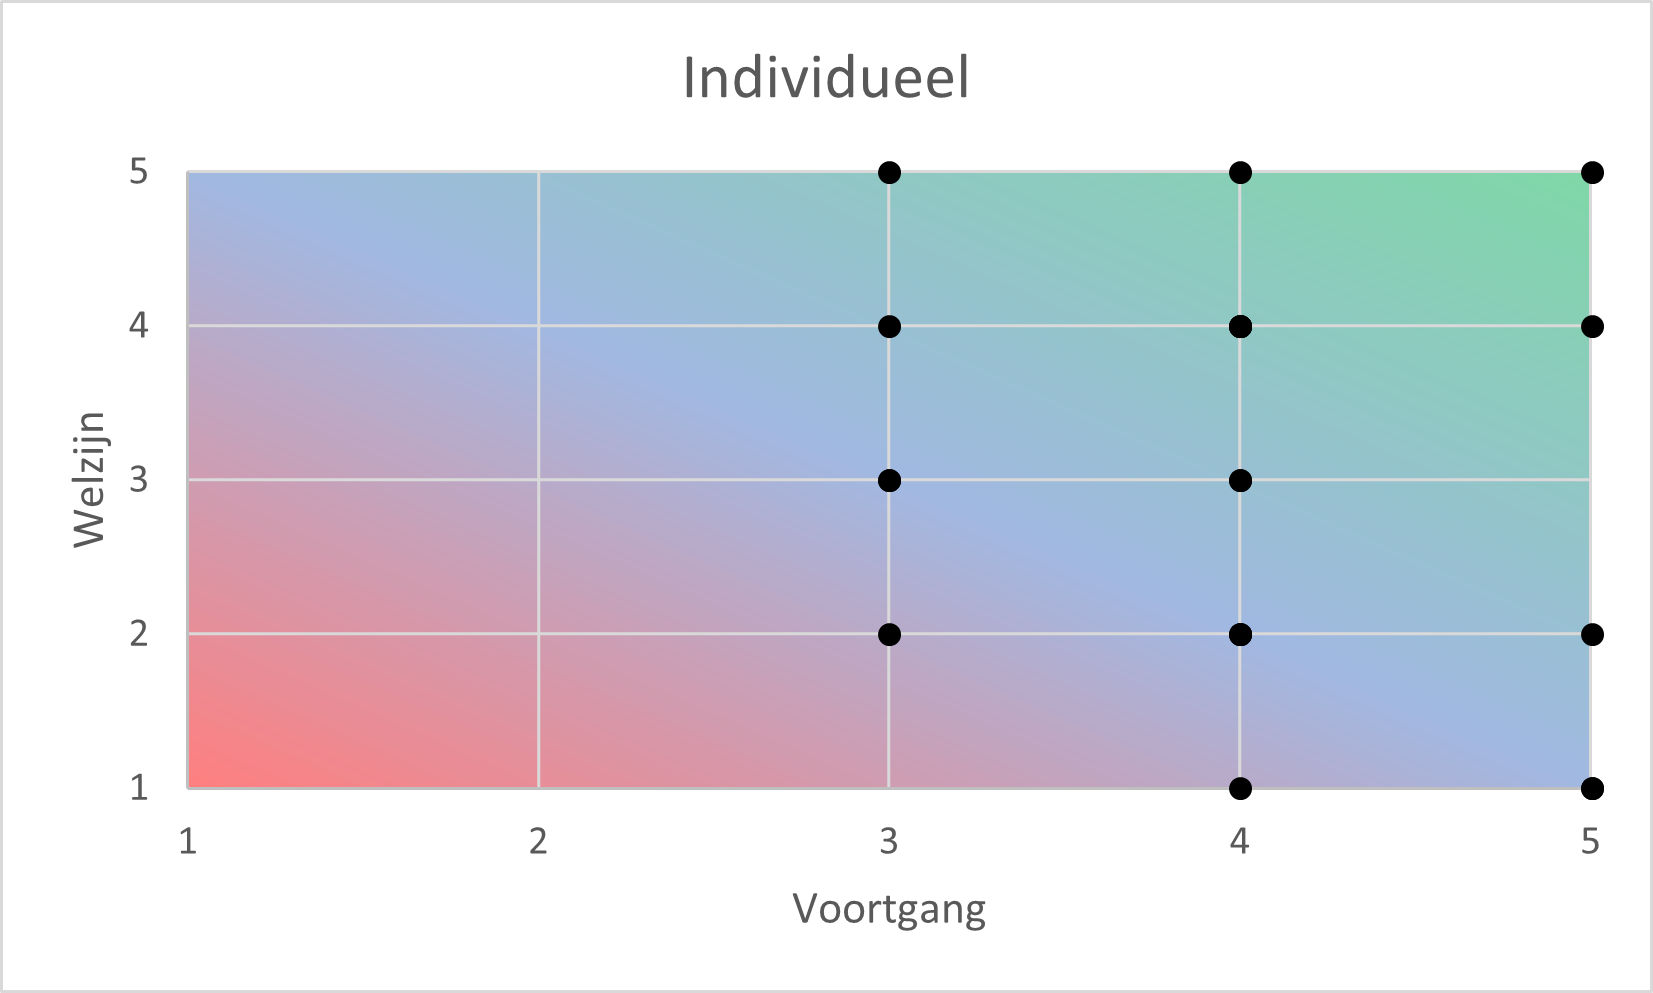
\includegraphics[width=\columnwidth]{individueel.png}
    \caption{Voortgang/welzijn-grafiek individueel}
    \label{Voortgang/welzijn-grafiek voor een individuele workflow. Overlappende punten worden hier niet speciaal weergegeven.}
\end{figure}

\begin{figure}[!hb]
    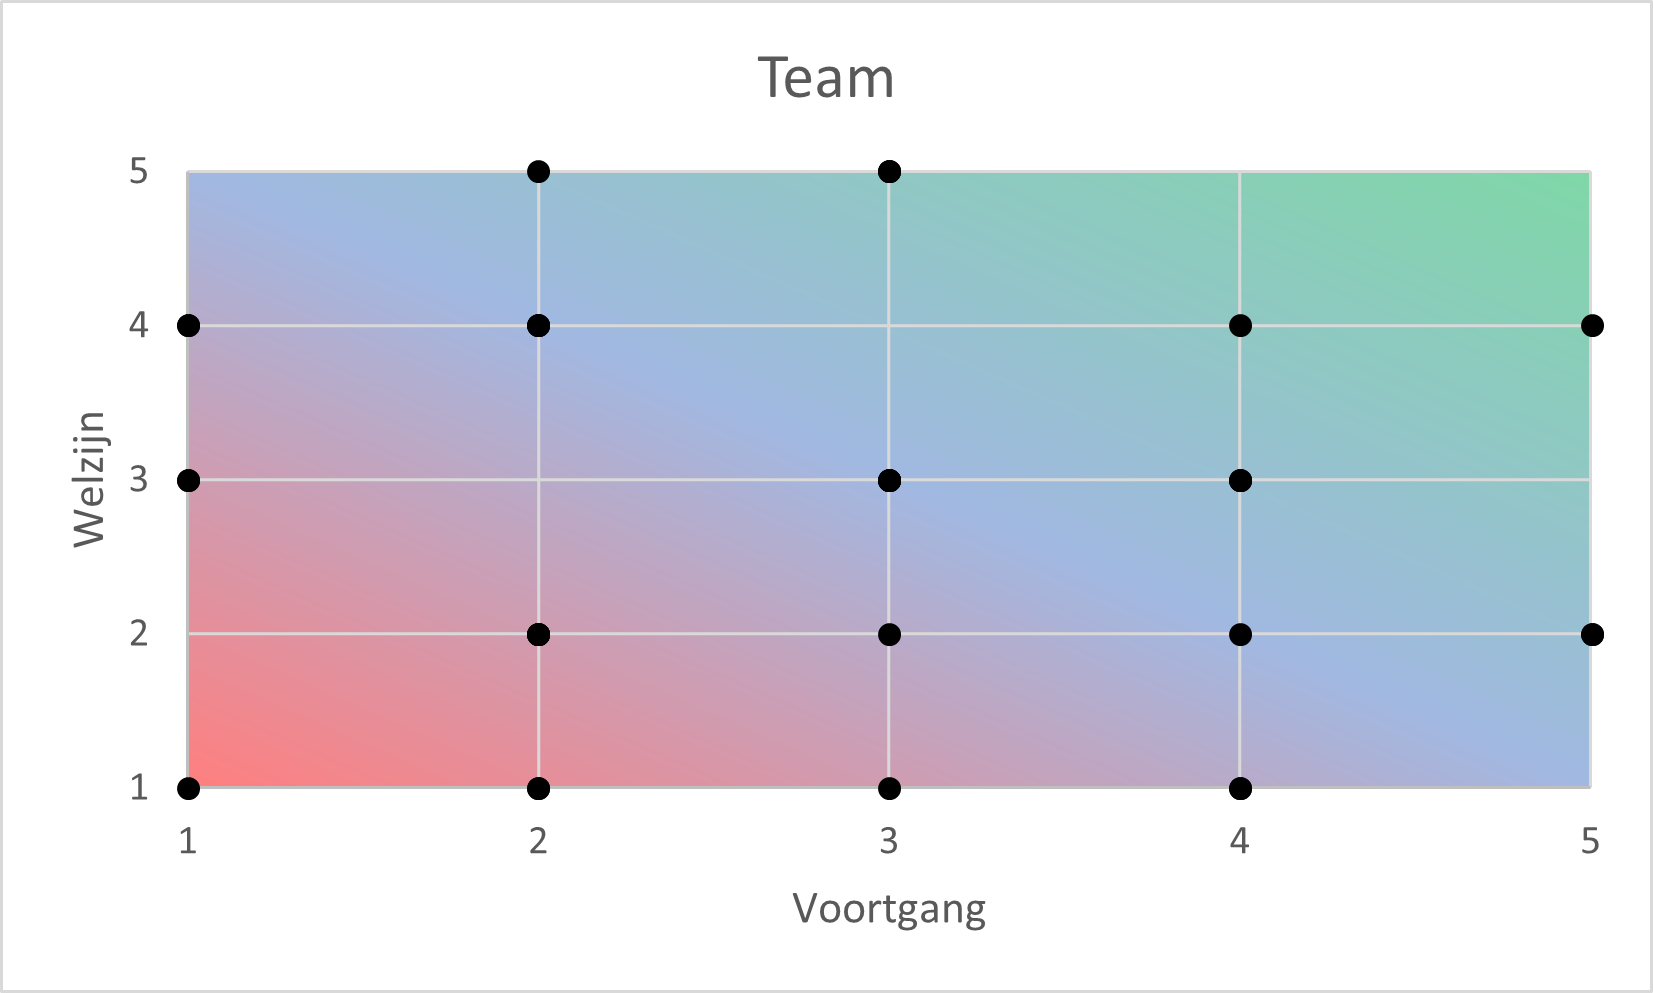
\includegraphics[width=\columnwidth]{team.png}
    \caption{Voortgang/welzijn-grafiek team}
    \label{Voortgang/welzijn-grafiek voor een teamsgebonden workflow. Overlappende punten worden hier niet speciaal weergegeven.}
\end{figure}

%---------- Verwachte conclusies ----------------------------------------------
\section{Verwachte conclusies}
\label{sec:verwachte_conclusies}

    
    Er wordt verwacht dat een individuele workflow voor voortgang zorgt ten koste van het welzijn van de developer. Tevens zou het werken in grote teams nefast zijn voor zowel de voortgang als het welzijn. De sprintduur zal omgekeerd evenredig zijn met de voortgang maar recht evenredig met het welzijn. De veranderlijkheid van requirements zal op zich weinig directe invloed hebben op zowel voortgang als welzijn.
    
    Er wordt tevens verwacht dat zowel de individuele workflow als de teamsgebonden workflow sterk onderhevig zijn aan externe factoren. Er zal echter te concluderen vallen dat er met een combinatie van beide implementaties, waar er in kleine teams van 2 of 3 mensen wordt gewerkt, een balans tussen beide kan bekomen worden. Hierbij kan er een sprintduur van 2 weken worden gehanteerd. De mate van veranderlijkheid van requirements zal echter meestal afhankelijk zijn van de klant en niet de implementatie van een Agile framework.
    
    Op basis van de verwachte data en de verwachte conclusies, zou er een framework kunnen voorgesteld worden waar elementen van Scrum in verwerkt worden, in combinatie met elementen van andere frameworks waar het werken in kleine groepen van 2 of 3 developers aangeraden wordt. Hierbij kan gedacht worden aan praktijken zoals Peer Programming\footnote{Praktijk waar 2 developers regelmatig elkaars werk doornemen en controleren teneinde zaken als het schrijven van duidelijke code} die bij frameworks zoals Extreme Programming (XP) prominent aanwezig zijn.
